\documentclass[twoside]{book}

% Packages required by doxygen
\usepackage{fixltx2e}
\usepackage{calc}
\usepackage{doxygen}
\usepackage[export]{adjustbox} % also loads graphicx
\usepackage{graphicx}
\usepackage[utf8]{inputenc}
\usepackage{makeidx}
\usepackage{multicol}
\usepackage{multirow}
\PassOptionsToPackage{warn}{textcomp}
\usepackage{textcomp}
\usepackage[nointegrals]{wasysym}
\usepackage[table]{xcolor}

% Font selection
\usepackage[T1]{fontenc}
\usepackage[scaled=.90]{helvet}
\usepackage{courier}
\usepackage{amssymb}
\usepackage{sectsty}
\renewcommand{\familydefault}{\sfdefault}
\allsectionsfont{%
  \fontseries{bc}\selectfont%
  \color{darkgray}%
}
\renewcommand{\DoxyLabelFont}{%
  \fontseries{bc}\selectfont%
  \color{darkgray}%
}
\newcommand{\+}{\discretionary{\mbox{\scriptsize$\hookleftarrow$}}{}{}}

% Page & text layout
\usepackage{geometry}
\geometry{%
  a4paper,%
  top=2.5cm,%
  bottom=2.5cm,%
  left=2.5cm,%
  right=2.5cm%
}
\tolerance=750
\hfuzz=15pt
\hbadness=750
\setlength{\emergencystretch}{15pt}
\setlength{\parindent}{0cm}
\setlength{\parskip}{3ex plus 2ex minus 2ex}
\makeatletter
\renewcommand{\paragraph}{%
  \@startsection{paragraph}{4}{0ex}{-1.0ex}{1.0ex}{%
    \normalfont\normalsize\bfseries\SS@parafont%
  }%
}
\renewcommand{\subparagraph}{%
  \@startsection{subparagraph}{5}{0ex}{-1.0ex}{1.0ex}{%
    \normalfont\normalsize\bfseries\SS@subparafont%
  }%
}
\makeatother

% Headers & footers
\usepackage{fancyhdr}
\pagestyle{fancyplain}
\fancyhead[LE]{\fancyplain{}{\bfseries\thepage}}
\fancyhead[CE]{\fancyplain{}{}}
\fancyhead[RE]{\fancyplain{}{\bfseries\leftmark}}
\fancyhead[LO]{\fancyplain{}{\bfseries\rightmark}}
\fancyhead[CO]{\fancyplain{}{}}
\fancyhead[RO]{\fancyplain{}{\bfseries\thepage}}
\fancyfoot[LE]{\fancyplain{}{}}
\fancyfoot[CE]{\fancyplain{}{}}
\fancyfoot[RE]{\fancyplain{}{\bfseries\scriptsize Generated by Doxygen }}
\fancyfoot[LO]{\fancyplain{}{\bfseries\scriptsize Generated by Doxygen }}
\fancyfoot[CO]{\fancyplain{}{}}
\fancyfoot[RO]{\fancyplain{}{}}
\renewcommand{\footrulewidth}{0.4pt}
\renewcommand{\chaptermark}[1]{%
  \markboth{#1}{}%
}
\renewcommand{\sectionmark}[1]{%
  \markright{\thesection\ #1}%
}

% Indices & bibliography
\usepackage{natbib}
\usepackage[titles]{tocloft}
\setcounter{tocdepth}{3}
\setcounter{secnumdepth}{5}
\makeindex

% Hyperlinks (required, but should be loaded last)
\usepackage{ifpdf}
\ifpdf
  \usepackage[pdftex,pagebackref=true]{hyperref}
\else
  \usepackage[ps2pdf,pagebackref=true]{hyperref}
\fi
\hypersetup{%
  colorlinks=true,%
  linkcolor=blue,%
  citecolor=blue,%
  unicode%
}

% Custom commands
\newcommand{\clearemptydoublepage}{%
  \newpage{\pagestyle{empty}\cleardoublepage}%
}

\usepackage{caption}
\captionsetup{labelsep=space,justification=centering,font={bf},singlelinecheck=off,skip=4pt,position=top}

%===== C O N T E N T S =====

\begin{document}

% Titlepage & ToC
\hypersetup{pageanchor=false,
             bookmarksnumbered=true,
             pdfencoding=unicode
            }
\pagenumbering{alph}
\begin{titlepage}
\vspace*{7cm}
\begin{center}%
{\Large My Project }\\
\vspace*{1cm}
{\large Generated by Doxygen 1.8.13}\\
\end{center}
\end{titlepage}
\clearemptydoublepage
\pagenumbering{roman}
\tableofcontents
\clearemptydoublepage
\pagenumbering{arabic}
\hypersetup{pageanchor=true}

%--- Begin generated contents ---
\chapter{File Index}
\section{File List}
Here is a list of all documented files with brief descriptions\+:\begin{DoxyCompactList}
\item\contentsline{section}{include/\hyperlink{global__vars_8hpp}{global\+\_\+vars.\+hpp} \\*Header gathering the global variables used in the Firmware }{\pageref{global__vars_8hpp}}{}
\item\contentsline{section}{src/\hyperlink{main_8cpp}{main.\+cpp} \\*Entry point for mbed OS }{\pageref{main_8cpp}}{}
\item\contentsline{section}{src/\hyperlink{sensInit_8cpp}{sens\+Init.\+cpp} \\*Thread initializing sensors read at the given frequency }{\pageref{sensInit_8cpp}}{}
\item\contentsline{section}{src/\hyperlink{UDPComm_8cpp}{U\+D\+P\+Comm.\+cpp} \\*Enables U\+DP communication between the target board and an external PC to perform Processor-\/\+In-\/the-\/\+Loop }{\pageref{UDPComm_8cpp}}{}
\end{DoxyCompactList}

\chapter{File Documentation}
\hypertarget{global__msgs_8hpp}{}\section{include/global\+\_\+msgs.hpp File Reference}
\label{global__msgs_8hpp}\index{include/global\+\_\+msgs.\+hpp@{include/global\+\_\+msgs.\+hpp}}
{\ttfamily \#include $<$mbed.\+h$>$}\newline
{\ttfamily \#include \char`\"{}common/mavlink.\+h\char`\"{}}\newline
Include dependency graph for global\+\_\+msgs.\+hpp\+:
\nopagebreak
\begin{figure}[H]
\begin{center}
\leavevmode
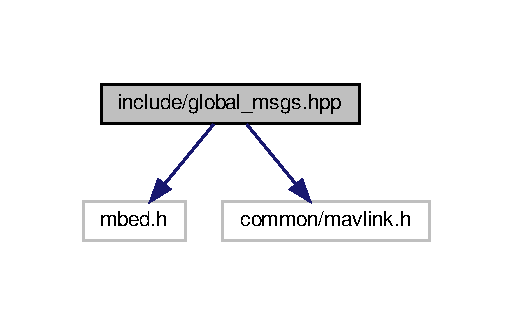
\includegraphics[width=246pt]{global__msgs_8hpp__incl}
\end{center}
\end{figure}
\subsection*{Variables}
\begin{DoxyCompactItemize}
\item 
mavlink\+\_\+attitude\+\_\+t \hyperlink{global__msgs_8hpp_a66611ecc414fa1c6fe5e014703d796cc}{att}
\end{DoxyCompactItemize}


\subsection{Variable Documentation}
\mbox{\Hypertarget{global__msgs_8hpp_a66611ecc414fa1c6fe5e014703d796cc}\label{global__msgs_8hpp_a66611ecc414fa1c6fe5e014703d796cc}} 
\index{global\+\_\+msgs.\+hpp@{global\+\_\+msgs.\+hpp}!att@{att}}
\index{att@{att}!global\+\_\+msgs.\+hpp@{global\+\_\+msgs.\+hpp}}
\subsubsection{\texorpdfstring{att}{att}}
{\footnotesize\ttfamily mavlink\+\_\+attitude\+\_\+t att}

Declaration and definition of used mavlink structs 
\hypertarget{global__vars_8hpp}{}\section{include/global\+\_\+vars.hpp File Reference}
\label{global__vars_8hpp}\index{include/global\+\_\+vars.\+hpp@{include/global\+\_\+vars.\+hpp}}


Header gathering the global variables used in the Firmware.  


{\ttfamily \#include $<$mbed.\+h$>$}\newline
{\ttfamily \#include \char`\"{}common/mavlink.\+h\char`\"{}}\newline
{\ttfamily \#include \char`\"{}feedback\+\_\+control.\+h\char`\"{}}\newline
{\ttfamily \#include \char`\"{}Servo.\+h\char`\"{}}\newline
This graph shows which files directly or indirectly include this file\+:
\nopagebreak
\begin{figure}[H]
\begin{center}
\leavevmode
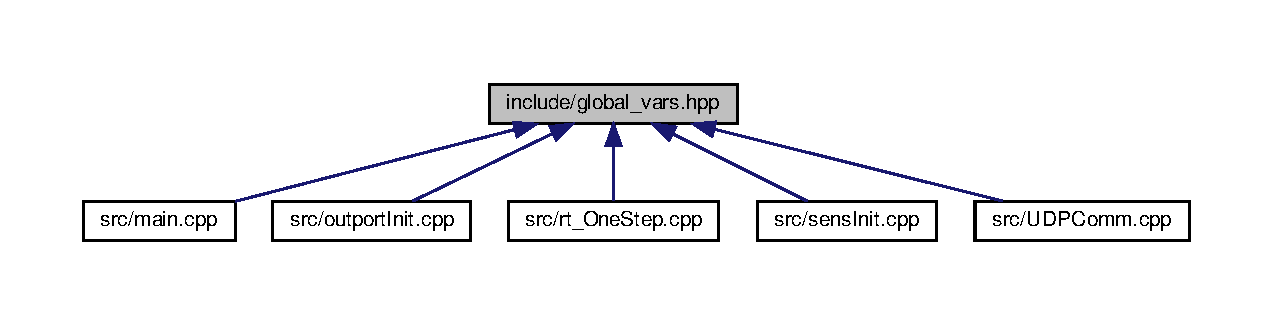
\includegraphics[width=199pt]{global__vars_8hpp__dep__incl}
\end{center}
\end{figure}
\subsection*{Variables}
\begin{DoxyCompactItemize}
\item 
Ext\+U\+\_\+feedback\+\_\+control\+\_\+T \hyperlink{global__vars_8hpp_a1bfda025b86a8da3a44e6b0923a256f2}{feedback\+\_\+control\+\_\+U}
\item 
Ext\+Y\+\_\+feedback\+\_\+control\+\_\+T \hyperlink{global__vars_8hpp_ae01be5449c13f73da04804c6c995d2ea}{feedback\+\_\+control\+\_\+Y}
\item 
\mbox{\Hypertarget{global__vars_8hpp_aaf3aa91f66e97e290265d2078ba3b1ad}\label{global__vars_8hpp_aaf3aa91f66e97e290265d2078ba3b1ad}} 
Semaphore {\bfseries sem\+Decode}
\item 
\mbox{\Hypertarget{global__vars_8hpp_a414bcf18f502e41c624ce447862af727}\label{global__vars_8hpp_a414bcf18f502e41c624ce447862af727}} 
Semaphore {\bfseries sem\+Encode}
\item 
\mbox{\Hypertarget{global__vars_8hpp_ac5d2bea44c6318454db0e2639a4efe95}\label{global__vars_8hpp_ac5d2bea44c6318454db0e2639a4efe95}} 
Servo {\bfseries servo1}
\item 
\mbox{\Hypertarget{global__vars_8hpp_ac158b76bc8e2f8f232c4b8a73d1a2cb2}\label{global__vars_8hpp_ac158b76bc8e2f8f232c4b8a73d1a2cb2}} 
Event\+Queue {\bfseries queue}
\end{DoxyCompactItemize}


\subsection{Detailed Description}
Header gathering the global variables used in the Firmware. 

Global variables are chosen upon u\+O\+RB because yes. 

\subsection{Variable Documentation}
\mbox{\Hypertarget{global__vars_8hpp_a1bfda025b86a8da3a44e6b0923a256f2}\label{global__vars_8hpp_a1bfda025b86a8da3a44e6b0923a256f2}} 
\index{global\+\_\+vars.\+hpp@{global\+\_\+vars.\+hpp}!feedback\+\_\+control\+\_\+U@{feedback\+\_\+control\+\_\+U}}
\index{feedback\+\_\+control\+\_\+U@{feedback\+\_\+control\+\_\+U}!global\+\_\+vars.\+hpp@{global\+\_\+vars.\+hpp}}
\subsubsection{\texorpdfstring{feedback\+\_\+control\+\_\+U}{feedback\_control\_U}}
{\footnotesize\ttfamily Ext\+U\+\_\+feedback\+\_\+control\+\_\+T feedback\+\_\+control\+\_\+U}

The I/O variables of the controller are used as extern since their name is the same if a Simulink project is used. This allows to keep the Firmware unchanged.\+External inputs \mbox{\Hypertarget{global__vars_8hpp_ae01be5449c13f73da04804c6c995d2ea}\label{global__vars_8hpp_ae01be5449c13f73da04804c6c995d2ea}} 
\index{global\+\_\+vars.\+hpp@{global\+\_\+vars.\+hpp}!feedback\+\_\+control\+\_\+Y@{feedback\+\_\+control\+\_\+Y}}
\index{feedback\+\_\+control\+\_\+Y@{feedback\+\_\+control\+\_\+Y}!global\+\_\+vars.\+hpp@{global\+\_\+vars.\+hpp}}
\subsubsection{\texorpdfstring{feedback\+\_\+control\+\_\+Y}{feedback\_control\_Y}}
{\footnotesize\ttfamily Ext\+Y\+\_\+feedback\+\_\+control\+\_\+T feedback\+\_\+control\+\_\+Y}

External outputs 
\hypertarget{main_8cpp}{}\section{src/main.cpp File Reference}
\label{main_8cpp}\index{src/main.\+cpp@{src/main.\+cpp}}


Entry point for mbed OS.  


{\ttfamily \#include $<$mbed.\+h$>$}\newline
{\ttfamily \#include $<$Serial.\+h$>$}\newline
{\ttfamily \#include $<$Ethernet\+Interface.\+h$>$}\newline
{\ttfamily \#include \char`\"{}global\+\_\+vars.\+hpp\char`\"{}}\newline
{\ttfamily \#include \char`\"{}common/mavlink.\+h\char`\"{}}\newline
{\ttfamily \#include \char`\"{}cntr\+Init.\+hpp\char`\"{}}\newline
{\ttfamily \#include \char`\"{}sens\+Init.\+hpp\char`\"{}}\newline
{\ttfamily \#include \char`\"{}outport\+Init.\+hpp\char`\"{}}\newline
{\ttfamily \#include \char`\"{}cli2.\+hpp\char`\"{}}\newline
Include dependency graph for main.\+cpp\+:\nopagebreak
\begin{figure}[H]
\begin{center}
\leavevmode
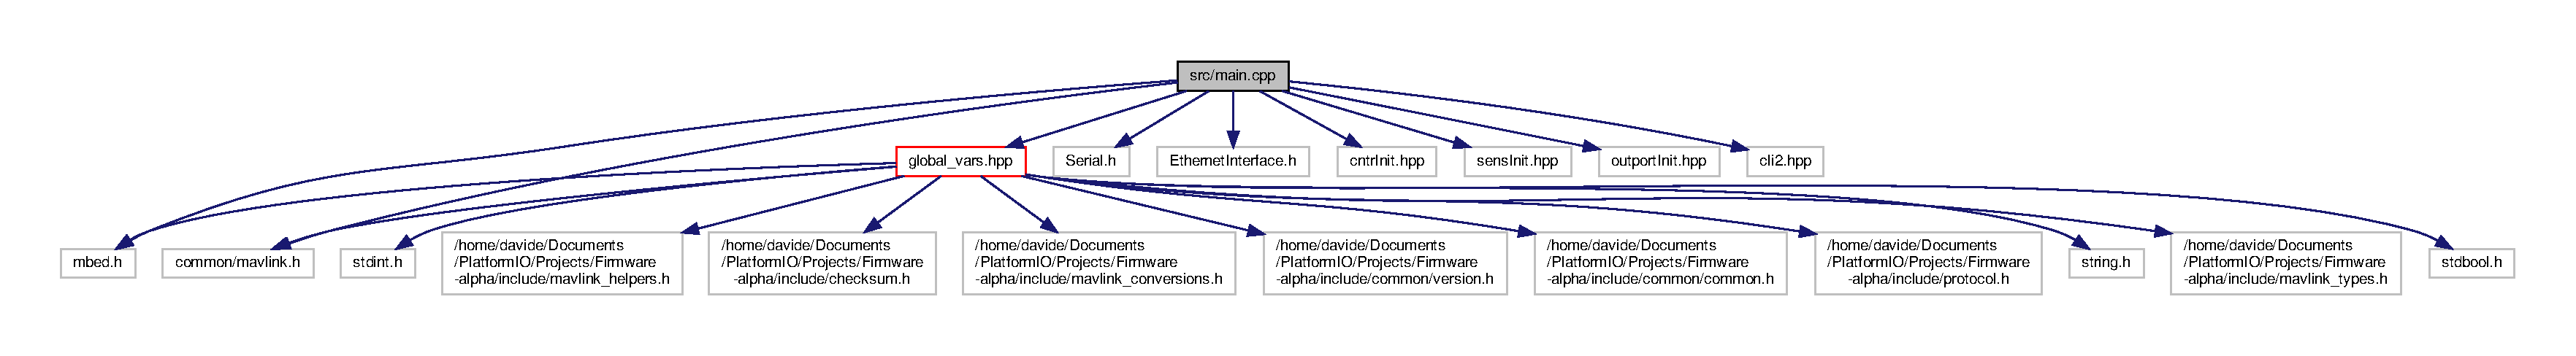
\includegraphics[width=350pt]{main_8cpp__incl}
\end{center}
\end{figure}
\subsection*{Variables}
\begin{DoxyCompactItemize}
\item 
Ext\+U\+\_\+feedback\+\_\+control\+\_\+T \hyperlink{main_8cpp_a1bfda025b86a8da3a44e6b0923a256f2}{feedback\+\_\+control\+\_\+U}
\item 
Ext\+Y\+\_\+feedback\+\_\+control\+\_\+T \hyperlink{main_8cpp_ae01be5449c13f73da04804c6c995d2ea}{feedback\+\_\+control\+\_\+Y}
\end{DoxyCompactItemize}


\subsection{Detailed Description}
Entry point for mbed OS. 

This script creates and spawns threads and declare global variables defined in the header \hyperlink{global__vars_8hpp}{global\+\_\+vars.\+hpp}. 

\subsection{Variable Documentation}
\mbox{\Hypertarget{main_8cpp_a1bfda025b86a8da3a44e6b0923a256f2}\label{main_8cpp_a1bfda025b86a8da3a44e6b0923a256f2}} 
\index{main.\+cpp@{main.\+cpp}!feedback\+\_\+control\+\_\+U@{feedback\+\_\+control\+\_\+U}}
\index{feedback\+\_\+control\+\_\+U@{feedback\+\_\+control\+\_\+U}!main.\+cpp@{main.\+cpp}}
\subsubsection{\texorpdfstring{feedback\+\_\+control\+\_\+U}{feedback\_control\_U}}
{\footnotesize\ttfamily Ext\+U\+\_\+feedback\+\_\+control\+\_\+T feedback\+\_\+control\+\_\+U}

The I/O variables of the controller are used as extern since their name is the same if a Simulink project is used. This allows to keep the Firmware unchanged.\+External inputs \mbox{\Hypertarget{main_8cpp_ae01be5449c13f73da04804c6c995d2ea}\label{main_8cpp_ae01be5449c13f73da04804c6c995d2ea}} 
\index{main.\+cpp@{main.\+cpp}!feedback\+\_\+control\+\_\+Y@{feedback\+\_\+control\+\_\+Y}}
\index{feedback\+\_\+control\+\_\+Y@{feedback\+\_\+control\+\_\+Y}!main.\+cpp@{main.\+cpp}}
\subsubsection{\texorpdfstring{feedback\+\_\+control\+\_\+Y}{feedback\_control\_Y}}
{\footnotesize\ttfamily Ext\+Y\+\_\+feedback\+\_\+control\+\_\+T feedback\+\_\+control\+\_\+Y}

External outputs 
\hypertarget{sensInit_8cpp}{}\section{src/sens\+Init.cpp File Reference}
\label{sensInit_8cpp}\index{src/sens\+Init.\+cpp@{src/sens\+Init.\+cpp}}


Thread initializing sensors read at the given frequency.  


{\ttfamily \#include $<$mbed.\+h$>$}\newline
{\ttfamily \#include \char`\"{}F\+X\+O\+S8700\+C\+Q.\+h\char`\"{}}\newline
{\ttfamily \#include \char`\"{}global\+\_\+vars.\+hpp\char`\"{}}\newline
{\ttfamily \#include \char`\"{}sens\+Init.\+hpp\char`\"{}}\newline
{\ttfamily \#include \char`\"{}Event\+Queue.\+h\char`\"{}}\newline
{\ttfamily \#include \char`\"{}Event.\+h\char`\"{}}\newline
Include dependency graph for sens\+Init.\+cpp\+:
\nopagebreak
\begin{figure}[H]
\begin{center}
\leavevmode
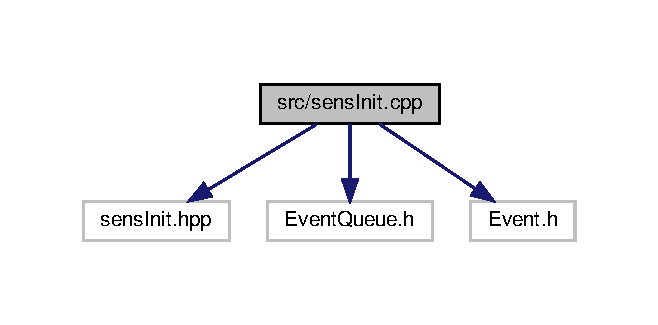
\includegraphics[width=350pt]{sensInit_8cpp__incl}
\end{center}
\end{figure}
\subsection*{Macros}
\begin{DoxyCompactItemize}
\item 
\mbox{\Hypertarget{sensInit_8cpp_afc65ba37dbbaa203d226e7fe6326adc5}\label{sensInit_8cpp_afc65ba37dbbaa203d226e7fe6326adc5}} 
\#define \hyperlink{sensInit_8cpp_afc65ba37dbbaa203d226e7fe6326adc5}{F\+X\+O\+S8700\+C\+Q\+\_\+\+F\+R\+EQ}~50
\begin{DoxyCompactList}\small\item\em Frequency at which the sensor is interrogated. \end{DoxyCompactList}\end{DoxyCompactItemize}


\subsection{Detailed Description}
Thread initializing sensors read at the given frequency. 

Creates a timer that calls an interrupt with the given frequency 
\hypertarget{UDPComm_8cpp}{}\section{src/\+U\+D\+P\+Comm.cpp File Reference}
\label{UDPComm_8cpp}\index{src/\+U\+D\+P\+Comm.\+cpp@{src/\+U\+D\+P\+Comm.\+cpp}}


Enables U\+DP communication between the target board and an external PC to perform Processor-\/\+In-\/the-\/\+Loop.  


{\ttfamily \#include $<$U\+D\+P\+Comm.\+hpp$>$}\newline
Include dependency graph for U\+D\+P\+Comm.\+cpp\+:
\nopagebreak
\begin{figure}[H]
\begin{center}
\leavevmode
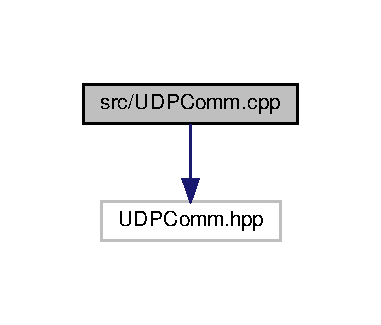
\includegraphics[width=183pt]{UDPComm_8cpp__incl}
\end{center}
\end{figure}
\subsection*{Functions}
\begin{DoxyCompactItemize}
\item 
\mbox{\Hypertarget{UDPComm_8cpp_a3a7725567b61c6b80243a548036bf6ca}\label{UDPComm_8cpp_a3a7725567b61c6b80243a548036bf6ca}} 
void {\bfseries U\+D\+P\+Comm} (void)
\end{DoxyCompactItemize}
\subsection*{Variables}
\begin{DoxyCompactItemize}
\item 
\mbox{\Hypertarget{UDPComm_8cpp_a6c3cca4bacec6b4aeb5cdaa86740614e}\label{UDPComm_8cpp_a6c3cca4bacec6b4aeb5cdaa86740614e}} 
uint8\+\_\+t {\bfseries in\+\_\+data} \mbox{[}M\+A\+V\+L\+I\+N\+K\+\_\+\+M\+A\+X\+\_\+\+P\+A\+C\+K\+E\+T\+\_\+\+L\+EN\mbox{]}
\item 
\mbox{\Hypertarget{UDPComm_8cpp_a4d0be1f983ac16fea15e5f5b3ca13f87}\label{UDPComm_8cpp_a4d0be1f983ac16fea15e5f5b3ca13f87}} 
uint8\+\_\+t {\bfseries out\+\_\+buf} \mbox{[}M\+A\+V\+L\+I\+N\+K\+\_\+\+M\+A\+X\+\_\+\+P\+A\+C\+K\+E\+T\+\_\+\+L\+EN\mbox{]}
\item 
\mbox{\Hypertarget{UDPComm_8cpp_a58a6aeee6d580249371bb554f6aeb6b1}\label{UDPComm_8cpp_a58a6aeee6d580249371bb554f6aeb6b1}} 
mavlink\+\_\+message\+\_\+t {\bfseries pos\+\_\+decoded}
\item 
\mbox{\Hypertarget{UDPComm_8cpp_a48be6085a723f7ef309f7f85875a4bcd}\label{UDPComm_8cpp_a48be6085a723f7ef309f7f85875a4bcd}} 
mavlink\+\_\+message\+\_\+t {\bfseries msg}
\item 
\mbox{\Hypertarget{UDPComm_8cpp_acdef7b92239f1e607ef6caa33a16d2ed}\label{UDPComm_8cpp_acdef7b92239f1e607ef6caa33a16d2ed}} 
mavlink\+\_\+status\+\_\+t {\bfseries status}
\item 
mavlink\+\_\+attitude\+\_\+t \hyperlink{UDPComm_8cpp_a66611ecc414fa1c6fe5e014703d796cc}{att}
\item 
\mbox{\Hypertarget{UDPComm_8cpp_a026404ba6f5a46eec468d3d538880b4a}\label{UDPComm_8cpp_a026404ba6f5a46eec468d3d538880b4a}} 
uint8\+\_\+t {\bfseries S\+Y\+S\+\_\+\+ID} = 1
\item 
\mbox{\Hypertarget{UDPComm_8cpp_ac78b977fae65f295acbf4ffc5e50b1e1}\label{UDPComm_8cpp_ac78b977fae65f295acbf4ffc5e50b1e1}} 
uint8\+\_\+t {\bfseries C\+O\+M\+P\+\_\+\+ID} = 1
\end{DoxyCompactItemize}


\subsection{Detailed Description}
Enables U\+DP communication between the target board and an external PC to perform Processor-\/\+In-\/the-\/\+Loop. 

Processor-\/\+In-\/the-\/\+Loop validation uses the external PC to simulate the physical model, its actuators and its sensors. The target board runs the firmware with full functionalities plus this thread that is responsible for sending/receiving simulation data to/from the external PC. The target board controls the model just as it was controlling the physical system.

\begin{DoxyNote}{Note}
The used communication protocol is Mavlink v2.\+0. 
\end{DoxyNote}


\subsection{Variable Documentation}
\mbox{\Hypertarget{UDPComm_8cpp_a66611ecc414fa1c6fe5e014703d796cc}\label{UDPComm_8cpp_a66611ecc414fa1c6fe5e014703d796cc}} 
\index{U\+D\+P\+Comm.\+cpp@{U\+D\+P\+Comm.\+cpp}!att@{att}}
\index{att@{att}!U\+D\+P\+Comm.\+cpp@{U\+D\+P\+Comm.\+cpp}}
\subsubsection{\texorpdfstring{att}{att}}
{\footnotesize\ttfamily mavlink\+\_\+attitude\+\_\+t att}

Declaration and definition of used mavlink structs 
%--- End generated contents ---

% Index
\backmatter
\newpage
\phantomsection
\clearemptydoublepage
\addcontentsline{toc}{chapter}{Index}
\printindex

\end{document}
